\section{Improve Programming Skills}
	\subsection{Reason to Choose}
		The topic of the Software Factory is completely new, which is the reason why I would like to improve my development skills in that kind of topics.

	\subsection{S.M.A.R.T.}
		\begin{SMART}
			\item[Specific] As my personal learning goal I want to improve my knowledge of the program language used in the project. The programming language used is not yet clear.
			\item[Measurable] This is measured by the result of the division of compiler errors by lines of code.
			\item[Attainable] Information about the programming language used may be found on the Internet but also in various books or ebooks.
			\item[Relevant] There are many programming languages but they can not all mastered. To have many options after graduation, you should have a lot of them already programmed.
			\item[Time-limited] The semester ends in January 2016 which is why I will have reached my goal by the end of January.
		\end{SMART}

	\subsection{S.T.A.R.R.}
		\begin{STARR}
			\item[Situation] We were using Xamarin Studio together with a student license to develop our product. Inside Xamarin the solution was written in C\# and separated into different projects for every platform. One project was for cross-platform development, which was also my main playground inside our project.
			\item[Task] I wanted to mainly improve my programming skills inside a cross-platform application.
			\item[Action] Inside the project I worked mainly inside the cross-platform project but also the iOS and the Android project got some attention. At first I built the complete main view structure and implemented it. For that the graph at the end of this sub section will show how does it work.

				Furthermore I invent together with Martijn Bonajo, a group member of my group, the MVVM pattern inside our cross-platform project.
				
			\item[Result] The results can be found in our group dossier in chapter 15 sections 1 to 25 and section 44.
			
				The compiler errors while I was programming was not so much I thought it would be. But unfortunately I had one compiler error every 100 lines of code.
			\item[Reflection] More or less I learned a lot about the MVVM Pattern used in Xamarin Studio.
		\end{STARR}
		
		\hspace*{4cm}
		\begin{turn}{90}
			\usetikzlibrary{trees}
			\tikzstyle{every node}=[draw=black,thick,anchor=west]
			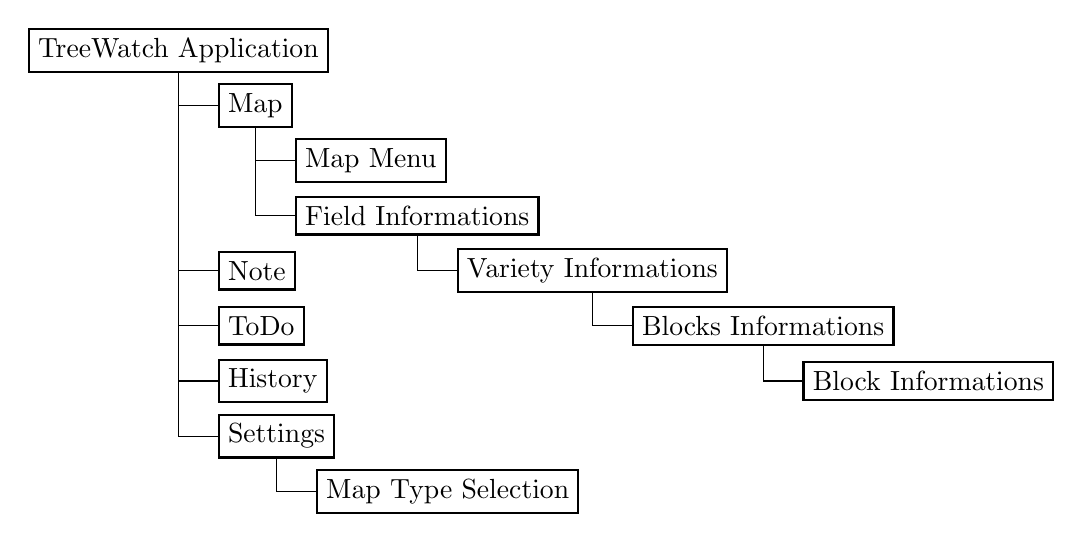
\begin{tikzpicture}[%
				grow via three points={one child at (0.5,-0.7) and
				two children at (0.5,-0.7) and (0.5,-1.4)},
				edge from parent path={(\tikzparentnode.south) |- (\tikzchildnode.west)}]
				\node {TreeWatch Application}
					child { node {Map}
				    	child { node {Map Menu}}
				    	child { node {Field Informations}
					    	child { node {Variety Informations}
				    			child { node {Blocks Informations}
							    	child { node {Block Informations}}
						    	}
				    		}
				    	}
					}
					child [missing] { node {Note}}
					child [missing] { node {Note}}
					child { node {Note}}
					child { node {ToDo}}
					child { node {History}}
					child { node {Settings}
				    	child { node {Map Type Selection}}
				    };
			\end{tikzpicture}
		\end{turn}